\documentclass[12pt]{article}
\usepackage[pdfborder={0 0 0.5 [3 2]}]{hyperref}%
\usepackage[left=1in,right=1in,top=1in,bottom=1in]{geometry}%
\usepackage[shortalphabetic]{amsrefs}%
\usepackage{amsmath}
\usepackage{enumerate}
\usepackage{enumitem}
\usepackage{amssymb}                
\usepackage{amsmath}                
\usepackage{amsfonts}
\usepackage{amsthm}
\usepackage{bbm}
\usepackage[table,xcdraw]{xcolor}
\usepackage{tikz}
\usepackage{float}
\usepackage{booktabs}
\usepackage{svg}
\usepackage{mathtools}
\usepackage{cool}
\usepackage{url}
\usepackage{graphicx,epsfig}
\usepackage{framed}
\usepackage{hyperref}  

\usetikzlibrary{automata,arrows,positioning,calc}
\DeclarePairedDelimiter\abs{\lvert}{\rvert}%
\DeclarePairedDelimiter\norm{\lVert}{\rVert}%
\DeclarePairedDelimiter\ceil{\lceil}{\rceil}
\DeclarePairedDelimiter\floor{\lfloor}{\rfloor}

\makeatletter
\renewcommand*\env@matrix[1][*\c@MaxMatrixCols c]{%
  \hskip -\arraycolsep
  \let\@ifnextchar\new@ifnextchar
  \array{#1}}
\makeatother

\newtheorem{theorem}{Theorem}[section]
\newtheorem{corollary}{Corollary}[theorem]
\newtheorem{proposition}[theorem]{Proposition}
\newtheorem{lemma}[theorem]{Lemma}

\theoremstyle{definition}
\newtheorem{definition}[theorem]{Definition}
\newtheorem{exercise}{Exercise}%
\newtheorem{problem}[exercise]{Problem}%
\newtheorem*{example}{Example}

\theoremstyle{remark}
\newtheorem*{question}{Question}
\newtheorem*{observation}{Observation}
\newtheorem*{remark}{Remark}

\graphicspath{ {images/} }

\setlength{\parindent}{0cm}
\renewcommand{\vec}[1]{\ensuremath{\mathbf{#1}}}

\def\noi{\noindent}
\def\T{{\mathbb T}}
\def\R{{\mathbb R}}
\def\N{{\mathbb N}}
\def\C{{\mathbb C}}
\def\Z{{\mathbb Z}}
\def\P{{\mathbb P}}
\def\E{{\mathbb E}}
\def\Q{\mathbb{Q}}
\def\ind{{\mathbb I}}

\def\cale{{\mathcal E}}
\def\cals{{\mathcal S}}
\def\calc{{\mathcal C}}
\def\caln{{\mathcal N}}
\def\calb{{\mathcal B}}
\def\calg{{\cal G}}

\def\ds{\displaystyle}
\def\ra{\rightarrow}
\newcommand{\conv}{\mbox{\rm conv}}
\newcommand{\spaan}{\mbox{\rm span}}
\newcommand{\deet}{\mbox{\rm det}}
\newcommand{\aff}{\mbox{\rm aff}}
\newcommand{\cl}{\mbox{\rm cl}}
\newcommand{\dimm}{\mbox{\rm dim}}
\newcommand{\sm}{\setminus}
\def\ci{\perp\!\!\!\perp}

\newcommand{\ink}{\rule{.5\baselineskip}{.55\baselineskip}}

\begin{document}

\setcounter{section}{3}
\section{Multivariate Distributions}

\subsection{Introduction}
Experimenters will often measure more than one quantity, and are often interested in the distribution of all observed quantities. As as example, a naturalist measures the height and weight of chimpanzees. They might be interested in the distribution of height-weight pairs. Since the distribution involves two quantities, we call it a \emph{bivariate distribution}. One question might be whether or not these two quantities are independent. (We suspect they are not, since a reasonable assumption is that taller chimpanzees tend to weigh more.)\\

Another important application of multivariate distributions is statistical sampling. Suppose $Y_1, Y_2, \dots, Y_n$ are $n$ successive trials of an experiment. Statisticians are interested in the distribution of $(Y_1, Y_2, \dots, Y_n)$, and can use information about this distribution to infer characteristics of the experiment or the population from which the experiment sampled.\\

In this section, we will primarily be interested in bivariate distributions, the probability distribution of two random variables. As before, we start with the discrete case and then consider the continuous case.

\subsection{Distribution of Two Discrete Random Variables}
First, let's define the joint probability distribution for a pair of discrete random variables.

\begin{framed}
\emph{Joint probabiltiy distribution, discrete case}\\
  \rule{\dimexpr\linewidth-2\fboxsep-2\fboxrule}{.1pt} \\
Let $Y_1$ and $Y_2$ be two discrete random variables. Then the \emph{joint distribution} of $Y_1$ and $Y_2$ is given by the function of two variables:
\begin{align*}
p(y_1, y_2) &= \P(Y_1 = y_1, Y_2 = y_2) & \text{for all possible pairs }(y_1, y_2)
\end{align*}
Sometimes this is called the \emph{joint probability mass function} (joint pmf). Note that $\P(Y_1 = y_1, Y_2 = y_2)$ means $\P(Y_1 = y_1 \cap Y_2 = y_2)$. This is standard notation for expressing the joint probability of two random variables. 
\end{framed}

We have already encountered one example of a bivariate distribution. Recall the distribution of the rolls of two standard, six-sided dice which we discussed several times in the section on discrete random variables. Let $X_1$ be the roll of the first die and $X_2$ the roll of the second die. Then since we have a discrete uniform distribution, the joint distribution of $X_1$ and $X_2$ is given by:
\begin{align*}
p(x_1, x_2) &= \frac{1}{36} & x_1, x_2 = 1, 2, 3, 4, 5, 6
\end{align*}

Just as in the case for a single discrete random variable, for a joint distribution of two discrete random variable, all the possible probabilties are nonnegative and they sum to 1.

\begin{framed}
Let $Y_1$ and $Y_2$ be discrete random variables with joint probability distribution $p(y_1, y_2)$. Then
\begin{align*}
0 \leq p(y_1, y_2) &\leq 1 \:\text{ for all }y_1, y_2 \\
\sum_{\text{all } (y_1, y_2} p(y_1, y_2) &= 1
\end{align*}
where the sum is taken over all possible pairs $(y_1, y_2)$.
\end{framed}

Just as in the case of a single discrete random variable, we can construct a valid joint probability distribution of two discrete random variables by assigning probabilities that add up to 1. Let $Y_1$ be a discrete random variable with $m$ possible output values, and $Y_2$ a discrete random variable with $n$ possible output values. Then there are $mn$ possible joint outputs of the pair of random variables. Each of the outputs is an ordered pair of the form $(y_1, y_2)$. If we make an $m$x$n$ table and assign probabilities to each of the $mn$ possible joint outputs so they add up to 1, we have constructed a joint probability distribution for the two discrete random variables $Y_1$ and $Y_2$.\\

Let's consider an example.

\begin{example}Imagine we surveyed Brown undergraduates and asked them two questions. 
\begin{enumerate}
\item Do you have an exam this week? 
\item How many cups of coffee have you drunk today?
\end{enumerate}
Let $X_1$ be the discrete random variable with values \{\texttt{yes}, \texttt{no}\} indicating whether or not a student has an exam this week. Let $X_2$ be the number of cups of coffee a student has drunk today. For simplicity, we will let $X_2$ take only the values \{0, 1, 2\} (Whether or not this is a realistic simplification is beyond the scope of this course!)\\

We can display the joint probabiltiy distribution for the pair $(X_1, X_2)$ in a 2 x 3 table. There are 6 possible values for the pair $(x_1, x_2)$. We can choose any probabilties for the six pairs as long as they sum to 1. One possible choice is shown in the table below.

\begin{table}[H]
\centering
\begin{tabular}{lllll}
                       &                                 &      & $X_2$    &                           \\ \cline{3-5}
                       &                                 & 0    & 1    & 2                         \\ \cline{3-5}
\multicolumn{1}{l|}{}  & \multicolumn{1}{l|}{\texttt{yes}}    & 2/20 & 3/20 & \multicolumn{1}{l|}{3/20} \\
\multicolumn{1}{l|}{$X_1$} & \multicolumn{1}{l|}{\texttt{no}} & 6/20 & 4/20 & \multicolumn{1}{l|}{2/20} \\ \cline{3-5}                  
\end{tabular}
\end{table}
You can verify that the six probabilities do indeed sum to 1.
\end{example}

\subsubsection{Marginal distribution}
Consider again a joint distribution $(Y_1, Y_2)$ of two discrete random variables with pmf $p(y_1, y_2)$. (You can think of the exam-coffee example above). $Y_1$ and $Y_2$ are themselves discrete random variables. What are their distributions? \\

Suppose we wish to find the distribution for $Y_1$ by itself. We call this the \emph{marginal distribution} of $Y_1$. Essentially what we want to do is take $Y_2$ out of the picture entirely. How do we do that? All we have to do is sum over all the possible values of $Y_2$! The probability that $Y_1 = y_1$ is the sum of $p(y_1, y_2)$ over all possible values $y_2$ that $Y_2$ can take; this is the marginal distribution of $Y_1$, and is written $p_1(y_1)$. Similarly, we can sum over all possible values $Y_1$ to get $p_2(y_2)$, the marginal distribution of $Y_2$. This is summarized below.

\begin{framed}
\emph{Marginal distribution, discrete random variables}\\
  \rule{\dimexpr\linewidth-2\fboxsep-2\fboxrule}{.1pt} \\
Let $Y_1$ and $Y_2$ be discrete random variables with joint probability distribution $p(y_1, y_2)$. Then the marginal distribution of $Y_1$ is given by:
\[
p_1(y_1) = \sum_{\text{all } y_2} p(y_1, y_2)
\]
and the marginal distribution of $Y_2$ is given by.
\[
p_2(y_2) = \sum_{\text{all } y_1} p(y_1, y_2)
\]
In both cases, we just sum the joint distribution over all the possibilities of the other random variable.
\end{framed}

Let's return to our example above.

\begin{example}In the exam-coffee example above, compute the marginal distributions for $X_1$ and $X_2$.\\

To find the marginal distributions for each variable, we sum over all the possibilities of the other variable. If the joint distribution is presented in a two-dimensional table, this ie easy. To find the marginal distribution of $X_2$, we sum the values in each column. The bottom row, which we will label ``total'', is the marginal distribution of $X_2$. Similarly, we can find the marginal distribution for $X_1$ by summing each row. The rightmost column, also labeled ``total'', is the marginal distribution for $X_2$. In fact, the marginal distribution is called ``marginal'' because its values lie in the margins of the joint distribution table.

\begin{table}[H]
\centering
\begin{tabular}{llllll}
                       &                                 &      & $X_2$   &                           &       \\ \cline{3-5}
                       &                                 & 0    & 1    & 2                         & total \\ \cline{3-5}
\multicolumn{1}{l|}{}  & \multicolumn{1}{l|}{\texttt{yes}}    & 2/20 & 3/20 & \multicolumn{1}{l|}{3/20} & 8/20  \\
\multicolumn{1}{l|}{$X_1$} & \multicolumn{1}{l|}{\texttt{no}} & 6/20 & 4/20 & \multicolumn{1}{l|}{2/20} & 12/20 \\ \cline{3-5}
                       & total                           & 8/20 & 7/20 & 5/20                      &      
\end{tabular}
\end{table}
You can check that the two marginal distributions sum to 1 and are thus valid probability distributions for discrete random variables.

\end{example}

\subsubsection{Conditional distirbution}
Suppose again we have a joint distribution $(Y_1, Y_2)$ of two discrete random variables with joint pmf $p(y_1, y_2)$. Another question we might ask is what is the distribution of $Y_1$ given that $Y_2 = y_2$. In other words, what is the conditional distribution of $Y_1$ given that $Y_2$ takes a specific value.\\

Let's look once more a the exam-coffee example to see how we can do this.

\begin{example}
In the exam-coffee example above,what is the distribution of the number of cups of coffee drunk today ($X_2$) given that a student has a midterm this week ($X_1$ = \texttt{yes})?\\

To do this, we look at the first row of the table, which corresponds to $X_1$ = \texttt{yes}. This is not a valid probability mass function, because the elements do not sum to 1. But we can fix that! All we have to do is divide by the marginal probability $p_1(\texttt{yes}) = \P(X_1 = \texttt{yes})$, which is conveniently located just to the right in the ``total'' column. If we do that, we get the conditional probability for $X_2$ given $X_1$ = \texttt{yes}, which we can write as $p(y_2 | \texttt{yes})$ or $p(y_2 | Y_1 = \texttt{yes})$:

\begin{table}[H]
\centering
\begin{tabular}{@{}ll@{}}
\toprule
y & $p(y | \text{midterm})$ \\ \midrule
0 & 2/8                                  \\
1 & 3/8                                  \\
2 & 3/8                                \\ \bottomrule
\end{tabular}
\end{table}
\end{example}

Now that we have seen an example, we will give the formal defintion of the conditional distribution of two discrete random variables.

\begin{framed}
\emph{Conditional distribution, discrete random variables}\\
  \rule{\dimexpr\linewidth-2\fboxsep-2\fboxrule}{.1pt} \\
Let $Y_1$ and $Y_2$ be discrete random variables with joint probability distribution $p(y_1, y_2)$. Let $p_2(y_2)$ be the marginal distribution of $Y_2$. Then the conditional distribution of $Y_1$ given $Y_2 = y_2$ is:
\[
p(y_1|y_2) = \P(Y_1 = y_1|Y_2 = y_2) = \frac{\P(Y_1 = y_1, Y_2 = y_2)}{\P(Y_2 = y_2)} = \frac{p(y_1, y_2)}{p_2(y_2)}
\]
where $p_2(y_2) > 0$. In words, the conditional distribution is the joint distribution divided by the marginal distribution. We can similarly define the conditional distribution of $Y_2$ given $Y_1 = y_1$.
\end{framed}

\subsubsection{Independence}
The final question to settle is independence. Roughly speaking, two random variables are independent of if the probabilities of each one are not affected by the value of the other one. The following will serve as our definition for independence of two discrete random variables.

\begin{framed}
\emph{Independence of discrete random variables}\\
  \rule{\dimexpr\linewidth-2\fboxsep-2\fboxrule}{.1pt} \\
Let $Y_1$ and $Y_2$ be discrete random variables with joint probability distribution $p(y_1, y_2)$. Let $p_1(y_1)$ and $p_2(y_2)$ be the marginal distributions of $Y_1$ and $Y_2$. Then $Y_1$ and $Y_2$ are independent if
\begin{align*}
p(y_1, y_2) &= p_1(y_1)p_2(y_2) & \text{for all }y_1, y_2
\end{align*}
In other words, two random variables are independent if their joint distribution is the product of the two marginal distributions.
\end{framed}

In the exam-coffee example above, using just about any pair of $y_1$ and $y_2$, we can show that $Y_1$ and $Y_2$ and not independent. Did we really expect them to be independent?

\subsection{Distribution of Two Discrete Continuous Variables}
We will essentially repeat the same discussion for a pair of continuous random variables. Since working with continuous random variables requires integration, this will require integration in two dimensions, i.e. multivariable calculus. Since it is likely that many of you have not taken multivariable calculus, all multivariable techniques will be taught as they are needed.

\subsubsection{Joint Probability Density}
Recall that in the discrete case, a probability distribution was described by a probability density function (pdf). For the joint distribution of two continuous random variable, we have a joint density funciton, which is the continuous analogue of the joint distribution function in the discrete case.

\begin{framed}
\emph{Joint probabiltiy density, continuous case}\\
  \rule{\dimexpr\linewidth-2\fboxsep-2\fboxrule}{.1pt} \\
Let $Y_1$ and $Y_2$ be two continuous random variables. Then the \emph{joint density} of $Y_1$ and $Y_2$ is a function of two variables $f(y_1, y_2)$ with the properties that:
\begin{enumerate}
\item $f(y_1, y_2) \geq 1$ for all $y_1, y_2$.
\item \[
\int_{-\infty}^\infty \int_{-\infty}^\infty f(y_1, y_2) dy_1 dy_2 = 1
\]
\end{enumerate}
\end{framed}
In other words, $f(y_1, y_2)$ is nonnegative and integrates to 1.\\

In the bivariate case, instead of finding the probabiltiy that a single variable lies in an interval $[a, b]$, we find the probability that a pair of random variables lies within a region of the plane. To do this, we integrate the joint density over that region.

\begin{framed}
\emph{Probability of an event, continuous bivariate case}\\
  \rule{\dimexpr\linewidth-2\fboxsep-2\fboxrule}{.1pt} \\
Let $Y_1$ and $Y_2$ be two continuous random variables with joint density $f(y_1, y_2)$. Let $A$ be a region of the plane. Then
\begin{align*}
\P((Y_1, Y_2) \in A) = 1 \int \int_A f(y_1, y_2) dy_1 dy_2
\end{align*}
\end{framed}
This notation may not be precise. Don't worry about it for now, we will do plenty of examples. Just remember the key idea: to find the probability that a pair of random variables lie in a region, integrate the joint density over that region.\\

The extra complication here is the double integral. Whereas a single integral is defined on a closed interval, a double integral is defined on a two-dimensional region of the plane. The key to success for any double integral problem is to draw the region of integration before doing anything else. Since this is so important, I will repeat it: always draw the region of integration!\\

We will learn how to handle this through a series of examples. We will keep coming back to this first example throughout this section.

\begin{example}Let $X$ and $Y$ be random variables with joint distribution function $f(x, y)$ given by:
\[
f(x, y) = \begin{cases} 
      k x y  & 0 \leq y \leq x \leq 1 \\
      0 & \textrm{otherwise}
   \end{cases}
\]

\begin{enumerate}
\item Find the value of $k$ such that $f(x, y)$ is a valid joint probability density function. \\

As defined above (and similar to the one-dimensional case), for a joint probability density function to be valid, its integral must be 1 over the region of integration, i.e.
\[
\int \int f(x, y) dx \: dy = 1
\]
The bounds of the density function are the following: $y \geq 0, y \leq x$, and $x \leq 1$. This describes the triangular region illustrated below.

\begin{figure}[H]
\centering
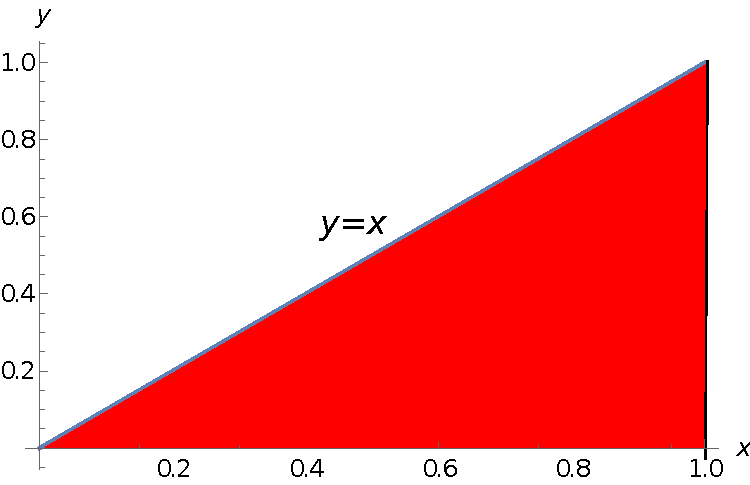
\includegraphics[width=8cm]{region1}
\end{figure}

Whenever we have a double integral, we have two choices when we do our integration. We can integrate in $x$ direction first, or we can integrate in the $y$ direction first. Both ways give the same answer, but sometimes one is easier than the other. We will show both of them here. \\

Let's start by integrating in the $y$ direction first. 
\begin{figure}[H]
\centering
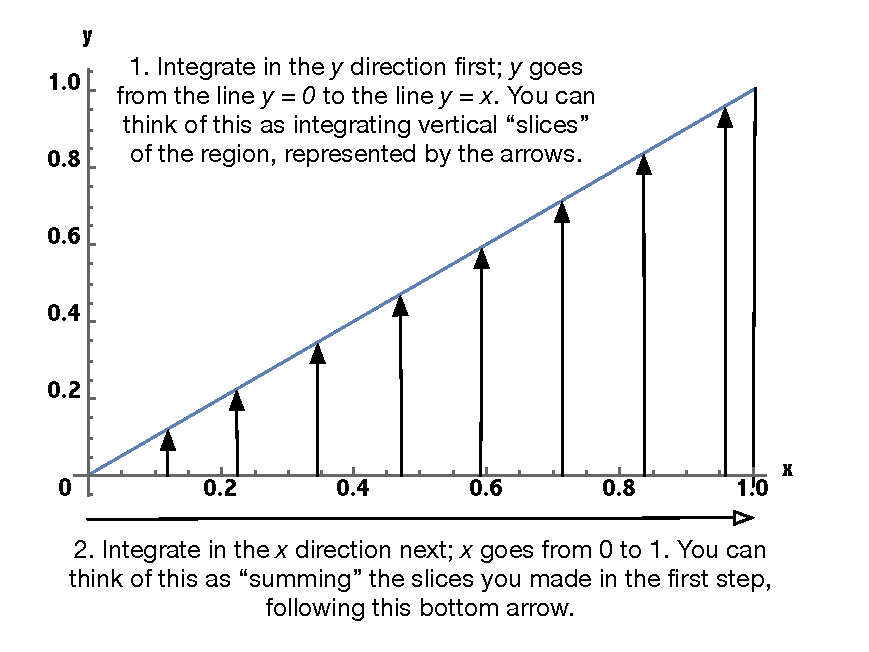
\includegraphics[width=10cm]{region1vertfirst.pdf}
\end{figure}
Following the directions on the picture above, we integrate $y$ first; $y$ goes from 0 to the diagonal line $y = x$, so those are the limits for the integral with respect to $y$ (inner integral). Note that the upper limit is a function of $x$. Each integral in $y$ is a vertical ``slice'' of our region. Then we integrate with respect to $x$. Imagining this as stacking our vertical slices side-by-side in the horizontal direction, $x$ goes from 0 to 1, so those are the limits for the integral with respect to $x$ (outer integral). Putting this together, we have:
\begin{align*}
1 &= \int_0^1 \int_0^x k x y \: dy dx \\
&= k \int_0^1 x \frac{y^2}{2} \Bigr|_0^x dx \\
&= \frac{k}{2} \int_0^1 x^3 dx \\
&= \frac{k}{2} \frac{x^4}{4} \Bigr|_0^1 = \frac{k}{8}  \\
\end{align*}
Multiplying by 8 gives us $k = 8$.\\

Let's do the integral the other way and verify to see if we get the same result. This time we integrate in the $x$ direction first.
\begin{figure}[H]
\centering
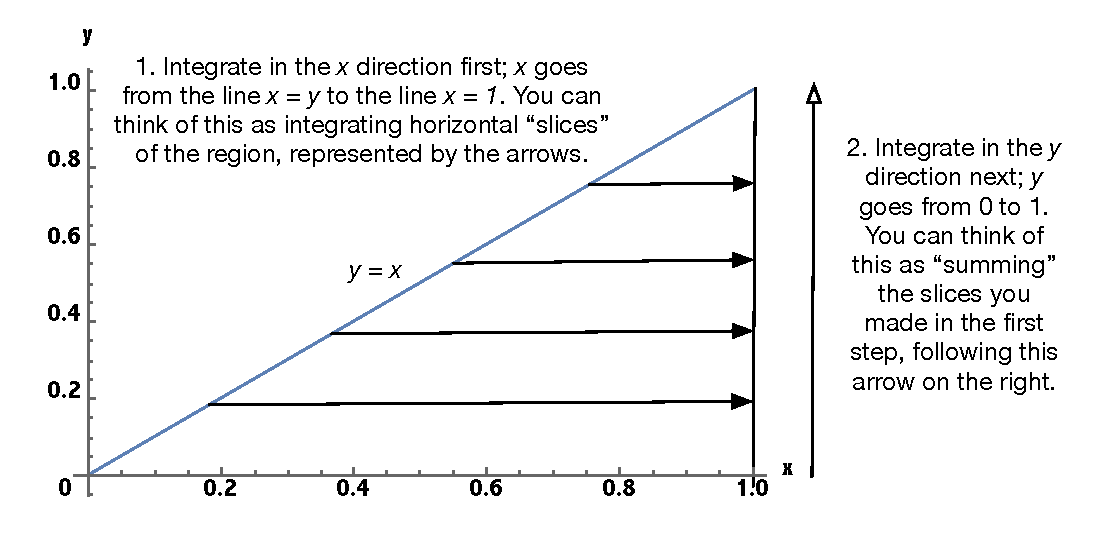
\includegraphics[width=10cm]{region1horizfirst}
\end{figure}
Once again following the directions on the picture above, we integrate $x$ first; $x$ starts at the diagonal line $y = x$ and goes to $x = 1$. The diagonal line has the eqution $y = x$, which we solve for $x$ to get $x = y$. Thus the lower limit is the function $x = y$. The upper limit is 1, so the limits of the integral with respect to $x$ (inner integral) are $y$ and 1. 
Each integral in $x$ is a horizontal ``slice'' of our region. Then we integrate with respect to $y$. Imagining this as stacking our horizontal slices one on top of the other in the vertical direction, $y$ goes from 0 to 1, so those are the limits for the integral with respect to $y$ (outer integral). Putting this together, we have:
\begin{align*}
1 &= \int_0^1 \int_y^1 k x y \: dx dy \\
&= k \int_0^1 y \frac{x^2}{2} \Bigr|_y^1 dy \\
&= \frac{k}{2} \int_0^1 y(1 - y^2) dy \\
&= \frac{k}{2} \int_0^1 (y - y^3) dy \\
&= \frac{k}{2} \left( \frac{y^2}{2} - \frac{y^4}{4} \right) \Bigr|_0^1 = \frac{k}{8}  \\
\end{align*}
We get the same answer! Which one was easier? \\

\item Find $\P(X < 0.6 \cap Y > 0.2)$.\\

Here we are finding the probability that the pair $(X, Y)$ falls in a specific region of the plane. The first step (as always) is to draw the region.
\begin{figure}[H]
\centering
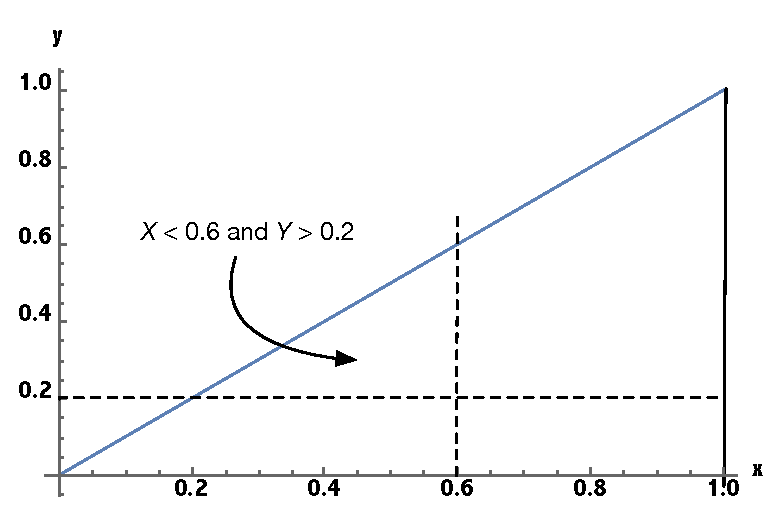
\includegraphics[width=8cm]{region1prob.pdf}
\end{figure}
From this picture, we get the limits of integration. Let's integrate in the $y$ direction first. Recall that we found that $k = 8$above. This gives us the integral:
\begin{align*}
\P(X < 0.6 \cap Y > 0.2) &= \int_{0.2}^{0.6} \int_{0.2}^x 8 x y \: dy dx
\end{align*}

This integral can be evaluated like the one above. The most important thing to know is how to set the problem up with the correct limits, but for completeness we will do the computation below.
\begin{align*}
\P(X < 0.6 \cap Y > 0.2) &= \int_{0.2}^{0.6} \int_{0.2}^x 8 x y \: dy dx \\
&= 8 \int_{0.2}^{0.6} x \frac{y^2}{2} \Bigr|_{0.2}^x dx \\
&= 4 \int_{0.2}^{0.6} (x^3 - 0.04x) dx \\
&= 4 \left( \frac{x^4}{4} - 0.04 \frac{x^2}{2} \right)\Bigr|_{0.2}^{0.6}\\
&= \left(0.6^4 - 0.2^4\right) - 0.08\left(0.6^2 - 0.2^2\right) \\
&= 0.1024
\end{align*}

We could also have integrated in the $x$ direction first.
\end{enumerate}
\end{example}

\subsubsection{Marginal Distribution}
Consider a joint distribution $(Y_1, Y_2)$ of two continuous random variables with joint density $f(y_1, y_2)$. $Y_1$ and $Y_2$ are themselves continuous random variables, and their distributions are called the \emph{marginal distributions} of $Y_1$ and $Y_2$. The probability densities of $Y_1$ and $Y_2$ are the \emph{marginal densities} of $Y_1$ and $Y_2$.\\

How do we find the marginal densities? Recall that for the discrete case, we summed over the other variable, e.g. to find the marginal density of $Y_1$, we summed the joint distribution over all the values $Y_2$ can take. Here we do the exact same thing, except we replace summation with integration. To get the marginal density of $Y_1$, we integrate the joint density $f(y_1, y_2)$ over $y_2$. The marginal density of $Y_1$ is written $f_1(y_1)$, and is a function of $y_1$ alone. (If after the integration you still have terms involving $y_2$, something went wrong.) Similarly, we can find the marginal density of $Y_2$.

\begin{framed}

\emph{Marginal density, continuous random variables}\\
  \rule{\dimexpr\linewidth-2\fboxsep-2\fboxrule}{.1pt} \\
Let $Y_1$ and $Y_2$ be continuous random variables with joint density $f(y_1, y_2)$. Then the marginal density of $Y_1$ is given by:
\[
f_1(y_1) = \int f(y_1, y_2) dy_2
\]
and the marginal density of $Y_2$ is given by.
\[
f_2(y_2) = \int f(y_1, y_2) dy_1
\]
In both cases, we integrate the joint density over the other random variable to remove it from the picture entirely. Sometimes we call this ``integrating out'' the other random variable.
\end{framed}

Let's return to the first example from the joint density section.

\begin{example}
Let $X$ and $Y$ be random variables with joint distribution function $f(x, y)$ given by:
\[
f(x, y) = \begin{cases} 
      8 x y  & 0 \leq y \leq x \leq 1 \\
      0 & \textrm{otherwise}
   \end{cases}
\]
\begin{enumerate}
\item Find the marginal densities for $X$ and $Y$.\\

Since our random variable are $X$ and $Y$, we will denote the two marginal densities by $f_X(x)$ and $f_Y(y)$. First, we find the marginal density for $X$ by integrating over $y$. Since we are integrating only in a single variable, there is only one choice for limits. Refer back to the picture of the region above. To integrate in $y$, we start at $y = 0$ and integrate until we reach the line $y = x$. Thus the limits of integration are 0 and $x$.

\begin{align*}
f_X(x) &= \int_0^x 8 x y \: dy \\
&= 8x \frac{y^2}{2} \Bigr|_0^x \\
&= 4 x^3
\end{align*}

With $Y$ out of the picture, the random variable $X$ is free to take values from 0 to 1. (The marginal distribution is one-dimensional, so there are no pesky regions to deal with!) The above expression for the marginal density is only valid for $0 \leq x \leq 1$. Outside that range, the marginal density is 0. Thus we write the marginal density $f_X(x)$ as:

\begin{align*}
f_X(x) &= \begin{cases}
  4 x^3 & 0 \leq x \leq 1 \\
  0 & \textrm{otherwise}
   \end{cases}
\end{align*}

It is important that we write the marginal density in this way so that we know that the $X$ is 0 outside $[0, 1]$. Since the marginal density is a valid probabiltiy density, you can check that it does in fact integrate to 1. Also note that the marginal density for $X$ is a function of $x$ alone; $y$ does not appear anywhere since we integrated it out!\\

Now we find the marginal density for $Y$ by integrating over $x$. The limits for $x$ are $x = 0$ and $x = y$. (See the picture of the region above if this is not clear.) 
\begin{align*}
f_Y(y) &= \int_y^1 8 x y \: dx \\
&= 8y \frac{x^2}{2} \Bigr|_y^1 \\
&= 4y(1 - y^2)
\end{align*}

With $X$ out of the picture, the random variable $Y$ can take values from 0 to 1, so we write the marginal density of $Y$ as
\begin{align*}
f_Y(y) &=  \begin{cases}
  4y(1 - y^2) & 0 \leq y \leq 1 \\
  0 & \textrm{otherwise}
   \end{cases}
\end{align*}

\item Find the expected values for $X$ and $Y$.\\

How do we find the expected values of $X$ and $Y$. We use the marginal densities and do the same thing we do every night, Pinky - try to take over the world! The marginal densities are just standard probability densities for continuous random variables; thus we find the expected values of $X$ and $Y$ using the marginal densities and the formula for the expected value of a continuous random variable.
\begin{align*}
\E(X) &= \int_{-\infty}^\infty f_X(x) dx \\
\E(Y) &= \int_{-\infty}^\infty f_Y(y) dy
\end{align*}

First we find the expected value for $X$. Notice that the limits of integration become 0 and 1, since that is the region where the marginal density is nonzero.

\begin{align*}
\E(X) &= \int_{-\infty}^\infty x f_X(x) dx \\
&= \int_0^1 x f_X(x) dx \\
&= \int_0^1 x \: 4 x^3 dx \\
&= 4 \int_0^1 x^4 dx \\
&= 4/5
\end{align*}

Similarly, we find the expected value of $Y$.
\begin{align*}
\E(Y) &= \int_{-\infty}^\infty y f_Y(y) dy \\
&= \int_0^1 y f_Y(y) \: dy \\
&= \int_0^1 y \: 4y(1 - y^2) dx \\
&= 4 \int_0^1 (y^2 - y^4) dx \\
&= 8/15
\end{align*}
\end{enumerate}
\end{example}

\subsubsection{Conditional Distribution}
Just as in the discrete case, we can talk about conditional distributions. In the continuous case, we will have a continuous density function. Suppose we have a joint distribution $(Y_1, Y_2)$ of two continuous random variables with conditional density $f(y_1, y_2)$. We might be interested in the distribution of $Y_1$ given that $Y_2 = y_2$. Since $Y_1$ is a continuous random variable, we will express this as a conditional probabiltiy density.\\

\begin{framed}
\emph{Conditional distribution, continuous random variables}\\
  \rule{\dimexpr\linewidth-2\fboxsep-2\fboxrule}{.1pt} \\
Let $Y_1$ and $Y_2$ be continuous random variables with joint probability density $f(y_1, y_2)$. Let $f_2(y_2)$ be the marginal density of $Y_2$. Then the conditional density of $Y_1$ given $Y_2 = y_2$ is:
\[
f(y_1|y_2) = \frac{f(y_1, y_2)}{f_2(y_2)}
\]
where $f_2(y_2) > 0$. As in the discrete case, the conditional density is the joint density divided by the marginal density. We can similarly define the conditional density of $Y_2$ given $Y_1 = y_1$.
\end{framed}
Note that the conditional density can (and often will) depend on the value of the random variable we are conditioning on. For example, $f(y_1|y_2)$ may depend on the value $y_2$. Furthermore, the range of valuee $y_1$ can take may also depend on $y_2$ (we will see this in the example below). Contrast this to the marginal density, where we eliminiate the other random variable entirely.\\

Once again, let's return to our example.

\begin{example}
Let $X$ and $Y$ be random variables with joint distribution function $f(x, y)$ given by:
\[
f(x, y) = \begin{cases} 
      8 x y  & 0 \leq y \leq x \leq 1 \\
      0 & \textrm{otherwise}
   \end{cases}
\]
\begin{enumerate}

\item Find the conditional density of $X$ given $Y = y$.\\

To find the conditional density $f(x|y)$, we divide the joint density $f(x, y)$ by the marginal density $f_Y(y)$. We found the marginal density above, so we have:
\begin{align*}
f(x|y) = \frac{f(x, y)}{f_Y(y)} = \frac{8 x y}{4y(1 - y^2) } = \frac{2x}{1 - y^2} 
\end{align*}
Note that this density does in fact depend on the value of $y$ we are conditioning on. However, we are not done. The bounds on the conditional density are important and must be specified. Referring back to the picture of the region, we note that if $Y = y$, then $X$ can only range from the diagonal line $y = x$ to 1, i.e. $X$ must be between $y$ and 1. Thus the conditional density of $X$ given $Y = y$ is given by:
\begin{align*}
f(x|y) &=  \begin{cases} 
      \frac{2x}{1 - y^2} & y \leq x \leq 1 \\
      0 & \textrm{otherwise}
   \end{cases}
\end{align*}

\item Find the conditional density of $Y$ given $X = x$.\\

Again, we divide the joint density by the marginal density, where we computed the marginal density $f_X(x)$ above.
\begin{align*}
f(y|x) = \frac{f(x, y)}{f_X(x)} = \frac{8 x y}{4x^3 } = \frac{2y}{x^2}  
\end{align*}
As with the other conditional density, this depends on $x$. The bounds of the conditional density will also depend on $x$. Looking at the picture of the region, if $X = x$, then $y$ can only range from 0 to the diagonal line $y = x$, i.e. $Y$ must be between 0 and $x$. Thus the conditional density is:
\begin{align*}
f(y|x) &=  \begin{cases} 
      \frac{2y}{x^2}  & 0 \leq y \leq x \\
      0 & \textrm{otherwise}
   \end{cases}
\end{align*}

\item Find the expected value of $X$ given $Y = y$.

A conditional density is just a probabiliy density of a continuous random variable, so we can find its expected value using the standard formula for the expected value of a continuous random variable.

\begin{align*}
E[X|Y = y] &= \int_{\infty}^{\infty} xf(x|y)dx\\
&= \int_y^1 x \frac{2x}{1 - y^2} dx \\
&= \frac{2}{1 - y^2} \int_y^1 x^2 \\
&= \frac{2}{1 - y^2}\frac{x^3}{3}\Bigr|_y^1 \\
&= \frac{2(1 - y^3)}{3(1 - y^2)}
\end{align*}
Note that we used the bounds on the conditional density in the second line above. Unsurprisingly, this depends on $y$.

\end{enumerate}
\end{example}

\subsubsection{Independence}
We have a similar defintion for independence in the case of continuous random variables.\\

\begin{framed}
\emph{Independence of continuous random variables}\\
  \rule{\dimexpr\linewidth-2\fboxsep-2\fboxrule}{.1pt} \\
Let $Y_1$ and $Y_2$ be continuous random variables with joint density $f(y_1, y_2)$. Let $f_1(y_1)$ and $f_2(y_2)$ be the marginal densities of $Y_1$ and $Y_2$. Then $Y_1$ and $Y_2$ are independent if
\begin{align*}
f(y_1, y_2) &= f_1(y_1)f_2(y_2) & \text{for all }y_1, y_2
\end{align*}
In other words, two continuous random variables are independent if their joint density is the product of the two marginal densities.
\end{framed}

In the example we have been looking at for the past three sections, the joint density is not the product of the marginal densities, so $X$ and $Y$ are not independent.\\

\subsubsection{Another Example}
Bivariate densities are important enough that we will provide more examples problems involving them.

\begin{example}Let $X$ and $Y$ be random variables with joint distribution function $f(x, y)$ given by:
\[
f(x, y) = \begin{cases} 
      c x  & 0 \leq x \leq y \leq 1 \\
      0 & \textrm{otherwise}
   \end{cases}
\]

\begin{enumerate}
\item Find the value of $c$ such that $f(x, y)$ is a valid joint probability density function.\\

The first step is always to draw the region.
\begin{figure}[H]
\centering
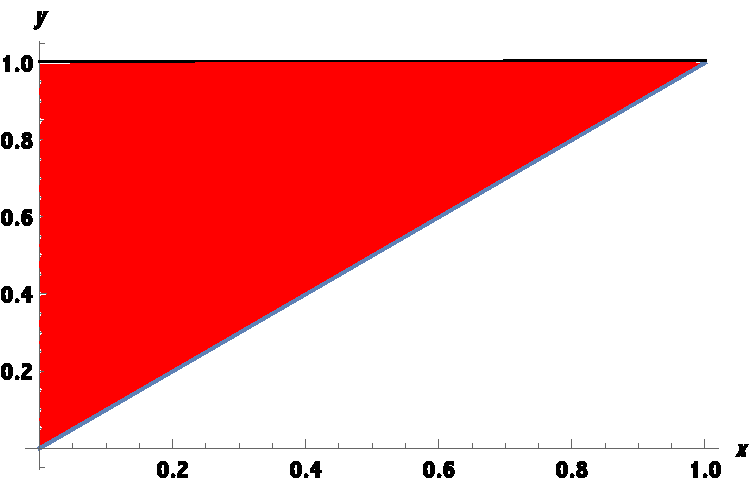
\includegraphics[width=8cm]{region2.pdf}
\end{figure}
To find the value of $c$, we integrate the joint density over the region and set the result equal to 1. We will integrate in the $x$ direction first since there's already an $x$ in the integrand and integrating in the $x$ direction first allows both lower limits to be 0 (the other choice would work fine too):
\begin{align*}
1 &= \int_0^1 \int_0^y c x dx dy \\
&= c \int_0^1 \frac{x^2}{2}\Bigr|_0^y dy \\
&= c \int_0^1 \frac{y^2}{2} dy \\
&= c \frac{y^3}{6}\Bigr|_0^1 \\
&= \frac{c}{6}
\end{align*}
Thus we find that $c = 6$ for this to be a valid joint probability density function.

\item Find the marginal densities for $X$ and $Y$.\\

To do this, we integrate out each random variable in turn. Be careful to get the correct limits of integration (refer back to the picture of the region early and often.) For the marginal density of $X$ we first integrate out $y$.
\begin{align*}
f_X(x) = \int_x^1 6 x dy \\
&= 6 x y\Bigr|_x^1 \\
&= 6 x(1 - x)
\end{align*}
With $Y$ removed from the picture, $X$ can freely range from 0 to 1, so the marginal density of $X$ is:
\begin{align*}
f_X(x) &= \begin{cases}
  6 x(1 - x) & 0 \leq x \leq 1 \\
  0 & \textrm{otherwise}
   \end{cases}
\end{align*}

For the marginal density of $Y$, we first integrate out $x$:
\begin{align*}
f_Y(y) &= \int_0^y 6 x dx \\
&= 3 x^2\Bigr|_0^y \\
&= 3 y^2
\end{align*}
Then, with $X$ removed from the picture, $Y$ can freely range from 0 to 1, so the marginal density of $Y$ is:
\begin{align*}
f_Y(y) &= \begin{cases}
  3 y^2 & 0 \leq y \leq 1 \\
  0 & \textrm{otherwise}
   \end{cases}
\end{align*}
It is important that you give the correct bounds for the marginal densities.

\item What is the expected value of $X$?

To find $\E(X)$, we use the formula for expected value of a continuous random variable with the marginal density for $X$.
\begin{align*}
\E(X) &= \int_{\infty}^\infty f_X(x) dx \\
&= \int_0^1 x 6 x(1 - x) dx \\
&= 6 \int_0^1 (x^2 - x^3) dx \\
&= 6 \left( \frac{x^3}{3} - \frac{x^4}{4} \right)\Bigr|_0^1 \\
&= 6\left(\frac{1}{3} - \frac{1}{4} \right)\\
&= \frac{1}{2}
\end{align*}
Similarly we can find the expected value of $Y$ using the marginal density for $Y$.

\item What is the conditional density for $X$ given $Y = y$?\\

To get the conditinal density $f(x|y)$, we first divide the joint density by the marginal density of $Y$:
\[
f(x|y) = \frac{ f(x, y) }{f_Y(y)} = \frac{ 6 x }{ 3 y^2 } = \frac{ 2 x }{ y^2 }
\]
What are the bounds on the conditional density? Refer back to the picture of the region above. Given that $Y = y$, $X$ can range from 0 to $y$, thus the conditional density is:
\begin{align*}
f(x|y) &=  \begin{cases} 
      \dfrac{ 2 x }{ y^2 } & 0 \leq x \leq y \\
      0 & \textrm{otherwise}
   \end{cases}
\end{align*}

\item What is the expected value of $X$ given $Y = y$?\\

Here, we use the formula for the expected value of a continuous random variable with the conditional density $f(x|y)$.
\begin{align*}
\E(X|Y = y) &= \int_{-\infty}^\infty f(x|y) dx \\
&= \int_0^y \dfrac{ 2 x }{ y^2 } dx \\
&= \dfrac{x^2}{y^2}\Bigr|0^y \\
&= \dfrac{y^2}{y^2} = 1
\end{align*}
It is interesting to note that in this case, the conditional expected value does not depend on $y$.

\end{enumerate}
\end{example}

\subsubsection{Joint Uniform Distribution}
Here we will consider the bivariate uniform distribution. Recall the for the continuous uniform distribution, the probability of an interval is proportional to its length. For the two-dimensional uniform distribution, the probability of a region is proportional to its area. Let's look at an example.

\begin{example}Let $X$ and $Y$ have a joint uniform distribution on the equilateral right triangle with sides of length 2. 
\begin{figure}[H]
\centering
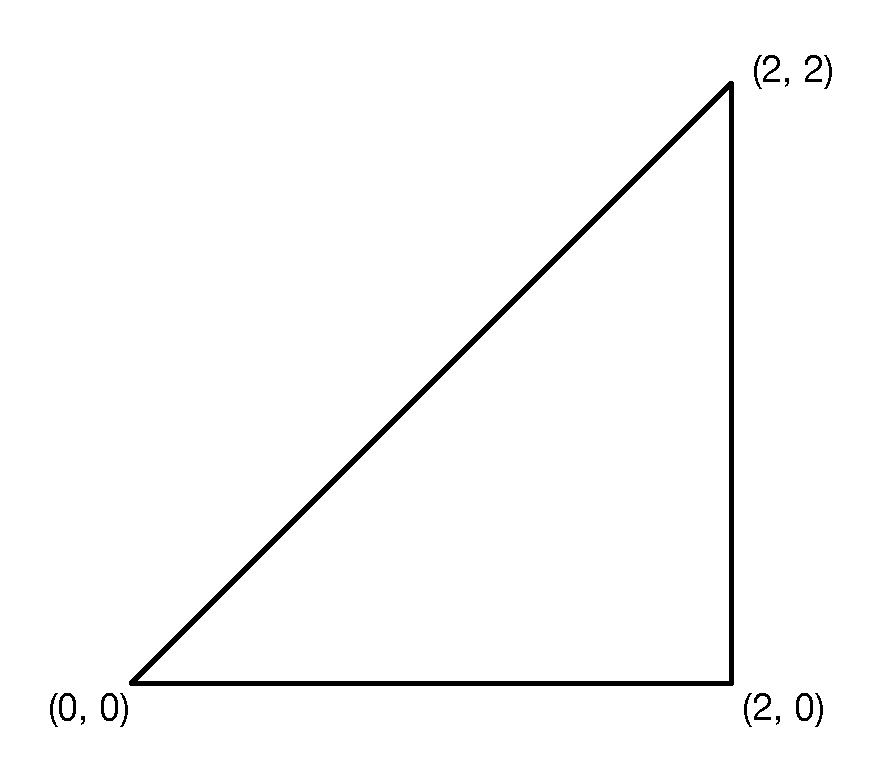
\includegraphics[width=5cm]{uniformtriangle}
\end{figure}

\begin{enumerate}
\item What is the probability that the pair $(X, Y)$ lies within the small square below (corners (1, 1) and (2, 0))?
\begin{figure}[H]
\centering
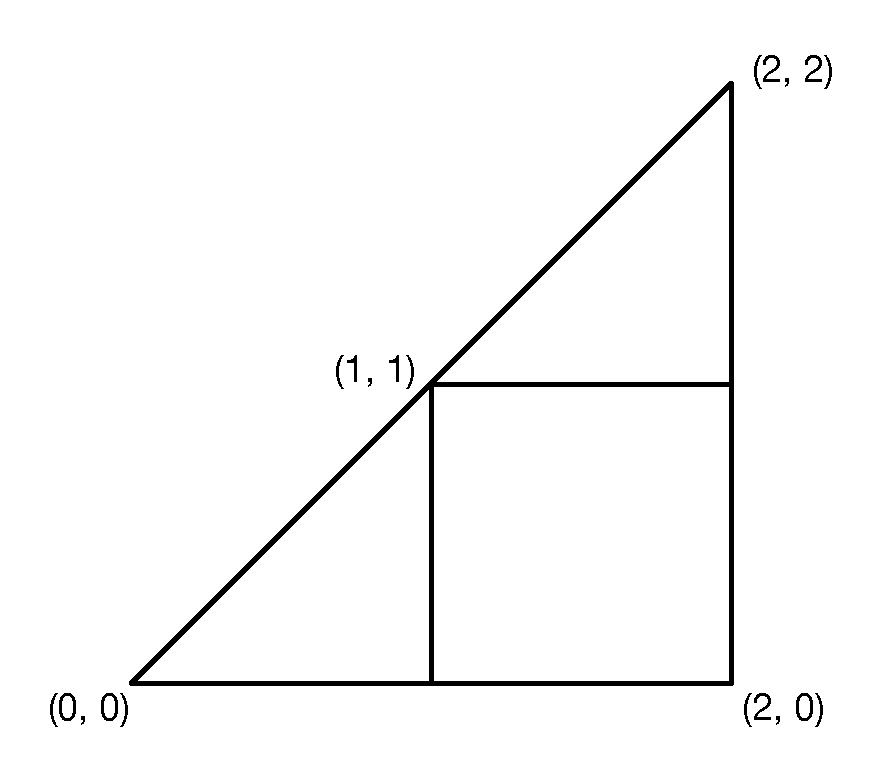
\includegraphics[width=5cm]{uniformtriangle2}
\end{figure}
The small square is half the area of the right triangle, so since this is the uniform distribution, the probability that $(X, Y)$ lies within the small square is 1/2.

\item What is the joint probability density of $(X, Y)$?\\

Recall that in the one-dimensional case, the uniform probability density is a constant. If $X \sim \text{Uniform}(a, b)$ then $X$ has density $f(x) = \frac{1}{b-a}$. This is just 1 divided by the length of the interval. This extends to the two-dimensional case. For a joint uniform distribution over a region, the joint uniform density is given by $1/A$, where $A$ is the area of the region. Just as in the one dimensional case, the joint uniform density is only defined on a region with \emph{finite} area. \\

Since the area of the triangle is 2, the joint uniform density is $f(x, y) = 1/2$. But we are not done! We need to specify the bounds of the uniform density, which will depend on the geometry of the region. Outside the region, the uniform density must be 0. Looking at the picture of the region above, we see that $y \geq 0$, $y \leq x$, and $x \leq 2$. Thus the joint density is:
\[
f(x, y) = \begin{cases} 
      \dfrac{1}{2}  & 0 \leq y \leq x \leq 2 \\
      0 & \textrm{otherwise}
   \end{cases}
\]

\item What are the marginal densities of $X$ and $Y$?

To find these, we take the joint density and integrate out each variable in turn. As always, we refer to the picture of the region to get the correct limits of integration. For the marginal density of $X$ we integrate over $y$:
\begin{align*}
f_X(x) &= \int_0^x \frac{1}{2} dy \\
&= \frac{1}{2} y\Bigr|_0^x \\
&= \frac{x}{2}
\end{align*}
With the correct bounds, the marginal density of $X$ is:
\begin{align*}
f_X(x) &= \begin{cases}
  \frac{x}{2} & 0 \leq x \leq 2 \\
  0 & \textrm{otherwise}
   \end{cases}
\end{align*}

Why are these the correct bounds for the marginal density? For the marginal density of $Y$ we integrate over $x$:
\begin{align*}
f_Y(y) &= \int_y^2 \frac{1}{2} dx \\
&= \frac{1}{2} x\Bigr|_y^1 \\
&= \frac{2 - y}{2}
\end{align*}
With the correct bounds, the marginal density of $Y$ is:
\begin{align*}
f_Y(y) &= \begin{cases}
 \frac{2 - y}{2} & 0 \leq y \leq 2 \\
  0 & \textrm{otherwise}
   \end{cases}
\end{align*}

\end{enumerate}
\end{example}
\end{document}
